\chapter{绪~~~论} % Representational learning 中枢神经系统
\label{c1}

经历了长期的自然选择进程,哺乳动物们演化出近似的大脑生理结构。尽管不同物种的大脑皮层有所差异,但其工作机制都表现出{层次性}(Hierarchical),{双向性}(Bidirectional),{专门化}(Specialization)和{综合化}(Integration)的特点\myciteup{liu2020vision}。在缺乏“无创”手段观察人类大脑的技术条件下,通过观察哺乳动物(如猫\myciteup{liu2020vision}、猕猴\myciteup{liu2020vision}等)的大脑,研究者们对大脑工作方式有了基本认识\myciteup{liu2020vision}。随着人们越来越清楚大脑的工作机制\myciteup{liu2020vision};这些感知、认知规律发挥着指导性作用,被用来开发人类智能\myciteup{liu2020vision},训练年轻医生应对临床信息的非确定性、优化诊断流程\myciteup{ liu2020vision},
甚至还作为基础理论,指导“人工智能”研究者们设计“模仿人类智能”的工具\myciteup{liu2020vision}。特别是“计算机视觉”技术的发展,就受益于心理学和认知神经科学的规律发现\myciteup{liu2020vision},现已被应用到包括了计算机辅助诊断的多个领域\myciteup{liu2020vision}。


\section{视觉上下文相关概念引入} %  概念引入
\label{c1:s1}
在探索大脑功能的进程中,人们对复杂感知和认知工作机制的认识,通常都依赖于更基础功能的发现。从发现单个神经元的生理功能开始,到逐渐探明大脑皮层上多个区域的功能,再到现在,了解到多个脑区之间协同的现象,有越来越多的研究者认识到了视觉上下文工作机制的作用\myciteup{liu2020vision}。
由于视觉信息占人类获取信息总体的八成以上\myciteup{liu2020vision},而且大脑皮层上负责处理视觉信息的脑区数目相应地比负责其它感官信息的更多\myciteup{liu2020vision},视觉上下文工作机制揭示的自适应性规律具有一定的普遍性。
为了清楚地阐述视觉上下文工作机制及其作用,避免相关概念在不同语境中的歧义,本节内容首先阐述相关概念。

图\ref{fig:1_2}展示了四种层级上的信息歧义或非确定性,分别是:(a)物理外观(Physical Appearance),A、B块的灰度相同\protect\footnotemark;(b)基本类别(Basic-Level Categories),是“打火机”,也可以是“手枪”\protect\footnotemark;(c)场景关联(Contextual Relations),黑色的目标是“吹风机”,也可以是“手电钻”\protect\footnotemark;(d)语义关联(Semantic Relations),是“A”,是“B”,也是“H”\protect\footnotemark。这些现象带来一个问题---如果相同的刺激只能激活同一个脑区,为什么会引发不同的感知和认知?传统的特征不变性理论无法对此做出合理解释。

\begin{figure}[tbp]
	\centering
	\subfigure[]{
		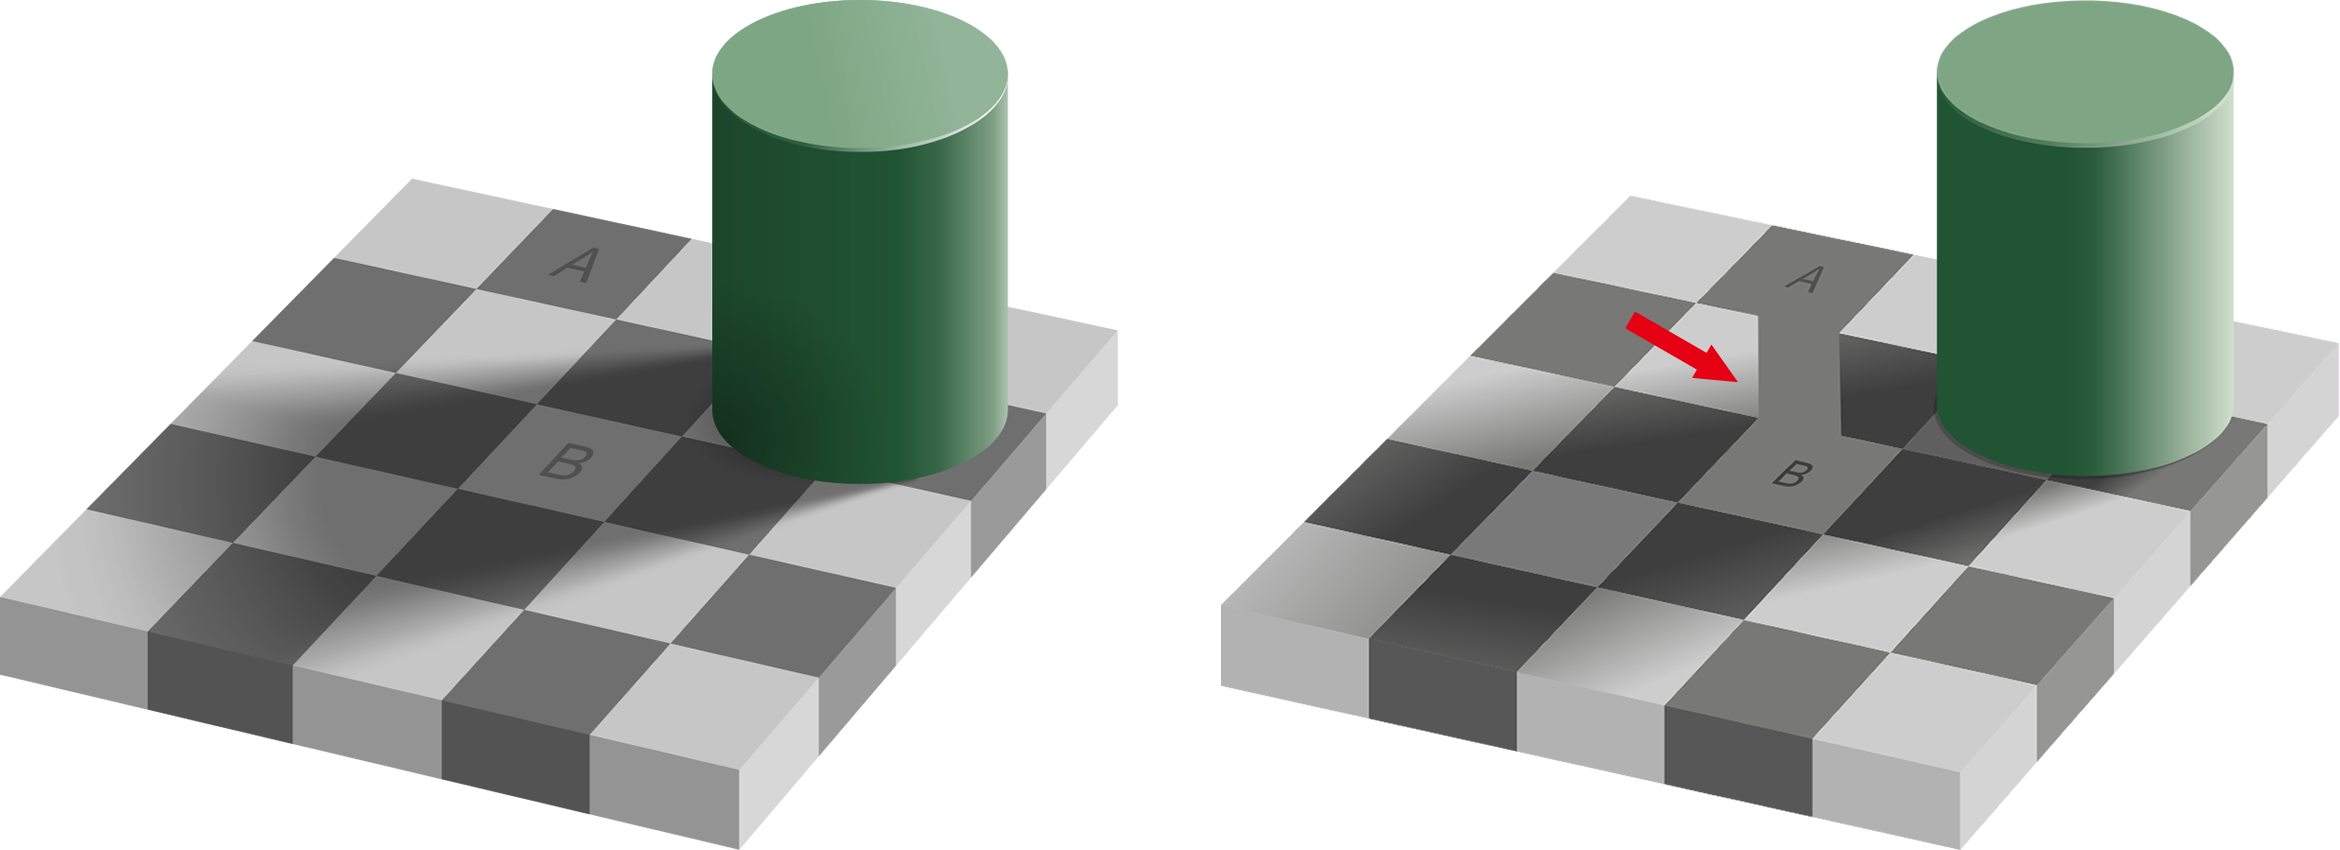
\includegraphics[height=0.165\textheight]{chapters/ch1_figs/checker_shadow}
	}
	\\
	\subfigure[]{
		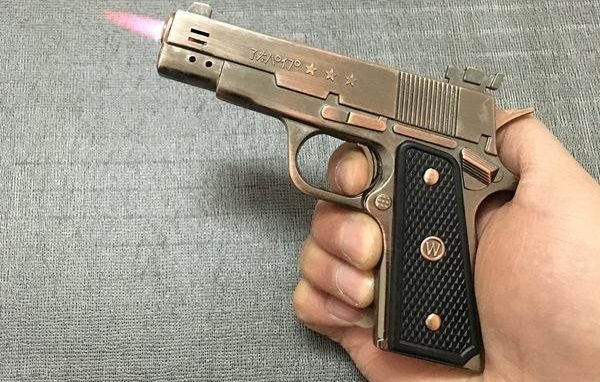
\includegraphics[height=0.165\textheight]{chapters/ch1_figs/lighter}
	}
	\\
	\subfigure[]{
		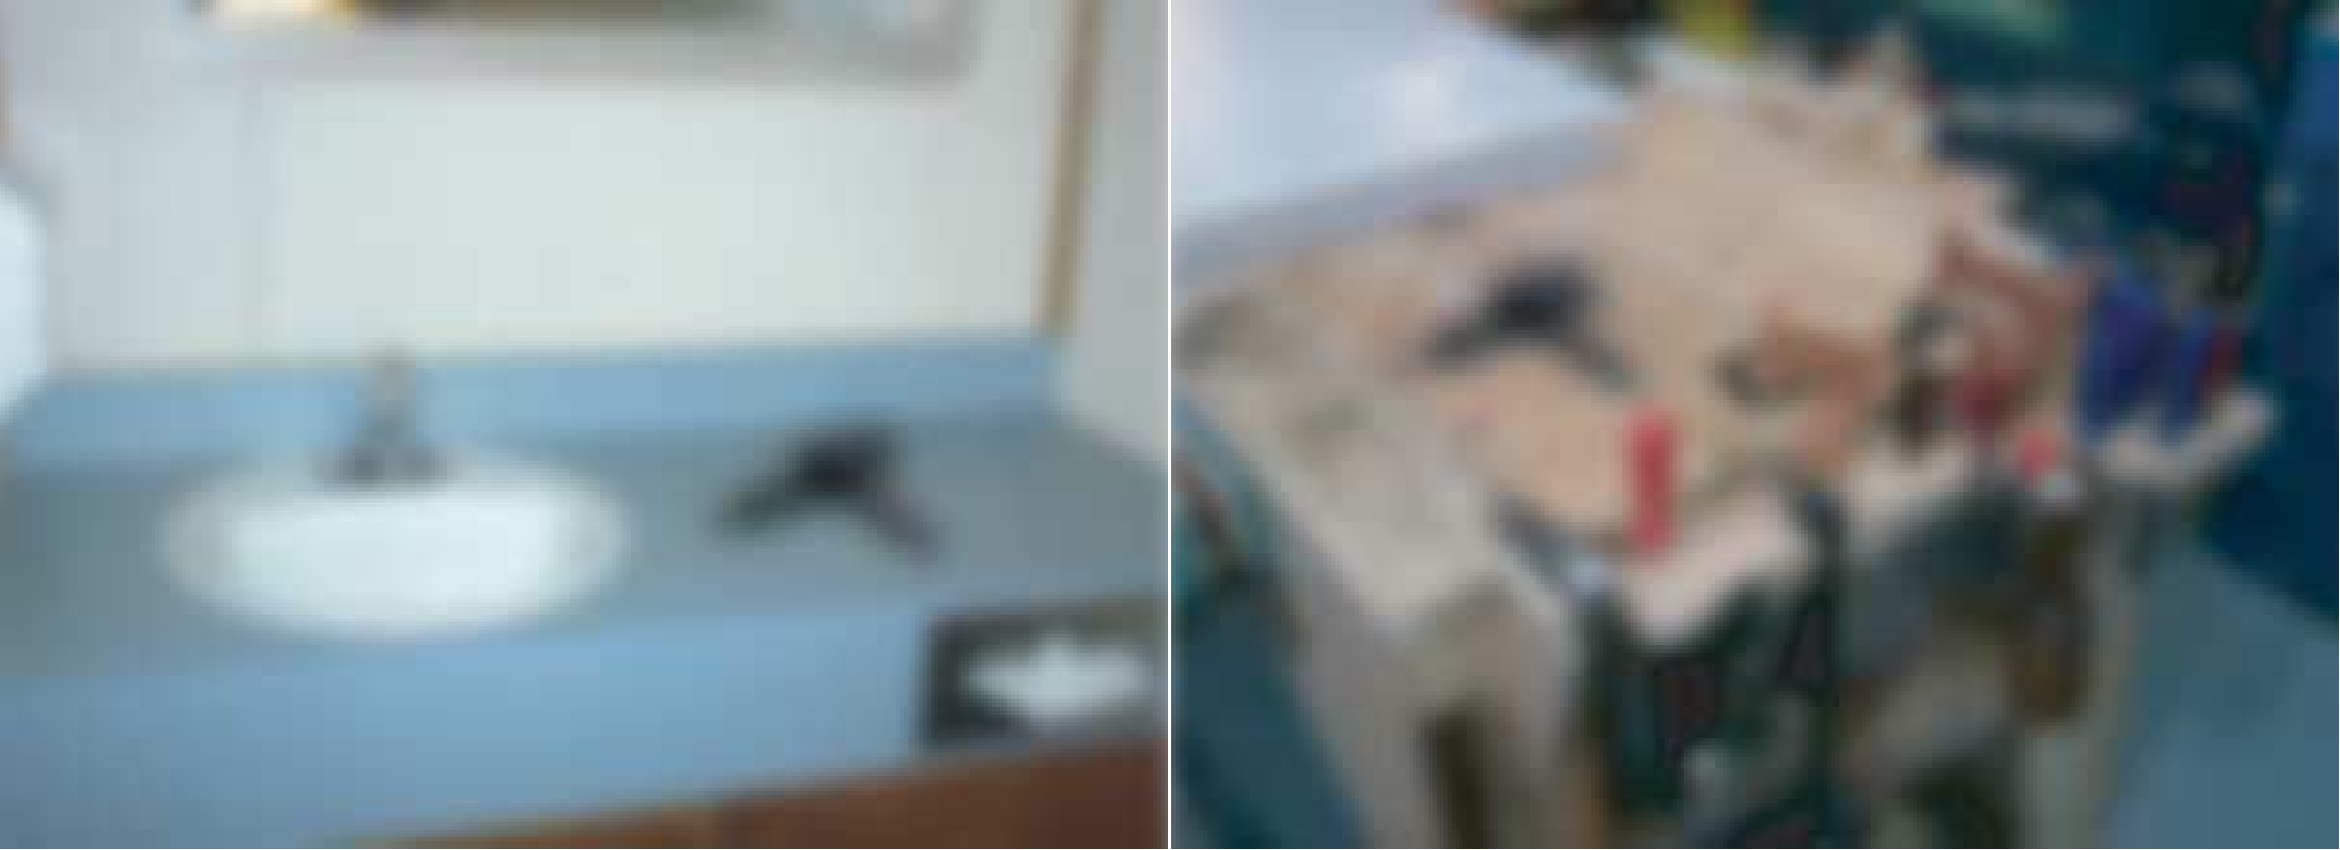
\includegraphics[height=0.165\textheight]{chapters/ch1_figs/context}
	}  
	\\
	\subfigure[]{
		
\includegraphics[height=0.165\textheight]{chapters/ch1_figs/letter}
	}
	\\
	\caption{\textbf{四种不同层级的视觉歧义性现象}} 
	\label{fig:1_2}
\end{figure}

\footnotetext[1]{图片来源:~\textit{https://en.wikipedia.org/wiki/Checker\_shadow\_illusion}}
\footnotetext[2]{图片来源:~\textit{https://www.dhgate.com/product/pkk-all-metal-pistol-double-fire-lighter/398614542.html\#s eo=WAP}}
\footnotetext[3]{图片来源:~\textit{https://www.nature.com/articles/nrn1476}}
\footnotetext[4]{图片来源:~\textit{https://www.ncbi.nlm.nih.gov/pmc/articles/PMC4441769/figure/F2}}



\section{论文组织结构}
\label{c1:s5}
本文总共包含七章内容,除去第\ref{c1}章“绪论”和第\ref{c7}章“总结与展望”以外,论文的主体部分主要有五章内容。它们分别介绍了构建上下文计算视觉模型的思路(第\ref{c2}章),以及提升了超像素聚类算法(第\ref{c3}章)、图像滤波算法(第\ref{c4}章)和神经纤维分类算法(第\ref{c6}章)自适应性。值得说明的是,本文提出的滤波算法在弥散加权影像的相位校正技术中也得到了成功的应用(第\ref{c5}章)。论文内容的主要框架如图\ref{fig:1_6}所示。


\usetikzlibrary{trees,calc}
%\pgfdeclarelayer{background}
%\pgfsetlayers{background,main}

	

    \tikzstyle{gb} = [rectangle, 
                      thick,
                      anchor=west,
                      inner sep=2pt,
                      rounded corners, 
                      text=white, 
                      font=\bfseries,
                      text centered, 
                      minimum width=4cm, 
                      minimum height=0.628cm, 
                      text centered, 
                      draw=black!70, 
                      fill=gray!70]

     \tikzstyle{bb} = [rectangle, 
                       thick,
                       anchor=west,
                       inner sep=2pt,
                       rounded corners, 
                       text=white, 
                       font=\bfseries,
                       text centered,  
                       minimum width=4cm, 
                       minimum height=0.628cm, 
                       text centered, 
                       draw=gray!70, 
                       fill=blue!40]
                       
%      \tikzstyle{ga} = [ultra thick,->,>=latex,lightgray,line width=0.07cm]


\begin{figure}[htbp]
	\centering
     \begin{tikzpicture}[
     grow via three points={
     	one child at (0.8,-0.7) and two children at (0.8,-0.7) and (0.8,-1.4)
     },
     edge from parent path={
     	($(\tikzparentnode\tikzparentanchor)+(.4cm,0pt)$) |- (\tikzchildnode\tikzchildanchor)
     },
     growth parent anchor=west,
     parent anchor=south west,% = \tikzparentanchor
     %   child anchor=west,%        = \tikzchildanchor
     %   every child node/.style={anchor=west}% already in "every node"
     ]
     \node [bb] {基于上下文的视觉感认知计算建模及其在核磁共振影像处理中的应用} 
     child [missing] {}
     child { node  [bb] {绪论 (第\ref{c1}章)} }
     %child [missing] {}
     child { node [bb] {视觉上下文的感认知计算建模 (第\ref{c2}章)} 
     child  { node  [gb, draw=none] {总结归纳了视觉上下文工作机制} }
     child  { node  [gb, draw=none] {提出了上下文计算视觉模型} }
     child { node [bb] {基于层次化超像素聚类的图像上下文生成方法 (第\ref{c3}章)} %[label={[xshift=6.0cm, yshift=-0.58cm, color=gray] Documentation for developers}]
     	child { node  [gb, draw=none] {自适应地生成超像素数目} }
     	child { node  [gb, draw=none] {以模仿视觉上下文形成的方式生成图像上下文} }
     	child { node  [gb, draw=none] {提出结构熵以衡量超像素编码影像结构信息的代价} } % 非均衡编码,带来更高的视觉编码效率
     		%child { node [draw=none] {\ldots}}
     	%child [missing] {}
     }
     % child [missing] {}
     % child [missing] {}
     child [missing] {}
     child [missing] {}
     child [missing] {}
     child { node [bb] {基于图像上下文的多核滤波算法(第\ref{c4}章)}
     	child { node [gb, draw=none] {几何化解释双边滤波器} }
     	child { node [gb, draw=none] {利用图像上下文自动生成滤波器参数,提升滤波器自适应性} }
     	%child [missing] {}    	
     	child { node [bb] {基于多核滤波器的空间自适应相位校正算法(第\ref{c5}章)}
     		% child { node [gb, draw=none]  {适用于处理弥散核磁张量影像中的非平稳噪声} }
     		% child { node [gb, draw=none]  {适用于应对弥散核磁张量影像中可变信噪比}  }     
     	} 
     }
     %child [missing] {}
     %child [missing] {}
     %child [missing] {}
     %child [missing] {}
     child [missing] {}
     child [missing] {}
     child [missing] {}
     child [missing] {}
     child { node  [bb]  {融合上下文信息的大脑神经纤维束分类算法 (第\ref{c6}章)}
     	child { node   [gb, draw=none] {利用图卷积网络提取神经纤维束的上下文几何特征} }
     	child { node   [gb, draw=none] {利用循环神经网络融合上下文几何特征和局部位置特征} }
        }
     }
    %child [missing] {}
    %child [missing] {}
    %child [missing] {}
    child [missing] {}
    child [missing] {}
    child [missing] {}
    child [missing] {}
    child [missing] {}
    child [missing] {}
    child [missing] {}
    child [missing] {}
    child [missing] {}
    child [missing] {}
    child [missing] {}
    child [missing] {}
    child [missing] {}
    child [missing] {}
    child { node [bb] {总结与展望 (第\ref{c7}章)} };     
     \end{tikzpicture}  
    \caption{\textbf{论文主要架构}}  
    \label{fig:1_6}  
\end{figure}